\chap{Changer les couleurs}

\sect{Colorer Thymio}

Créons un programme qui affiche deux couleurs différentes sur le dessus de Thymio lorsque les boutons avant ou arrière sont touchés, et deux autres couleurs sous et sur les côtés de Thymio lorsque les boutons gauche ou droite sont touchés.

{\raggedleft \hfill Programme: \bu{colors.aesl}}

Nous avons besoin de quatre paires d'événement-action.
Il y a quatre événements --- toucher l'un des quatre boutons --- et une action couleur est associée avec chaque événement.
Notez la différence entre le bloc \blksm{action-colors-up} et le bloc \blksm{action-colors-down}. Le premier des deux change la couleur affichée sur le dessus de Thymio alors que le deuxième change la couleur affichée sur le dessous et sur les côtés. Le deuxième bloc a deux marques noires qui représentent les roues du robot.

Ce programme est illustré sur la \cref{fig.colors-a}.

Quelles couleurs seront affichées? Pour les premières trois actions, le slider d'une couleur a été glissé tout à droite alors que les autres sont restés à gauche.
Ces actions affichent donc respectivement purement du rouge, du bleu et du vert.
L'action associée avec le bouton gauche mixe du rouge et du vert, ce qui produit donc du jaune.
Vous pouvez voir que le fond de l'action couleur se colorie en fonction de la position des \textit{sliders}, cela vous montre de quelle couleur sera Thymio!

Lancez le programme (icône \blksm{run}) et vérifiez que toucher les boutons change les couleurs du robot.
La \cref{fig.front} montre Thymio illuminé en rouge sur le dessus et la \cref{fig.bottom} montre Thymio illuminé en vert sur le dessous.

\exercisebox{\thechapter.1}{
Expérimentez avec les sliders pour voir quelles couleurs peuvent être affichées.
}

\trickbox[Information]{
\gr{color-cubes}{1}
En mixant ensemble du rouge, du vert et du bleu, vous pouvez faire n'importe quelle couleur !
}

\sect{Éteindre les lumières}

Modifions maintenant le programme pour que les lumières s'éteignent lorsque le bouton central est touché. Nous allons avoir besoin de deux paires événement-action, une pour éteindre les lumières du dessus de Thymio et une autre pour les lumières du dessous. En faisant glisser tous les \textit{sliders} sur la gauche, comme sur la \cref{fig.colors-b}, la lumière sera éteinte.
Vous voyez que l'événement est le même, toucher sur le bouton central, mais l'action associée est différente, éteindre les lumières du haut ou du bas.
N'oubliez pas de lancer le programmer en cliquant sur l'icône \blksmpure{run}.
À l'avenir, il sera implicite qu'il vous faudra lancer chaque programme en cliquant sur cet icône, nous ne vous le dirons plus.

\vfill

\importantbox[De multiples paires événement-action]{
\begin{itemize}[noitemsep,nosep,leftmargin=*]
\item Lorsqu'un programme est lancé, toutes les paires d'événement-action sont actives.
\item Il est possible d'avoir plusieurs fois le même événement mais il faut que le bloc d'action associé soit différent.
\item Si l'événement et le bloc d'action sont identiques dans plusieurs paires, VPL vous indiquera qu'il y a une erreur (zone 3 dans la \cref{fig.vplgui}).
Vous ne pourrez pas lancer le programme tant qu'il y a des erreurs.
\end{itemize}
}

\begin{figure}
    \centering
    \subfigure[Changer les couleurs lorsqu'un bouton flèche est touché]{
		\label{fig.colors-a}
		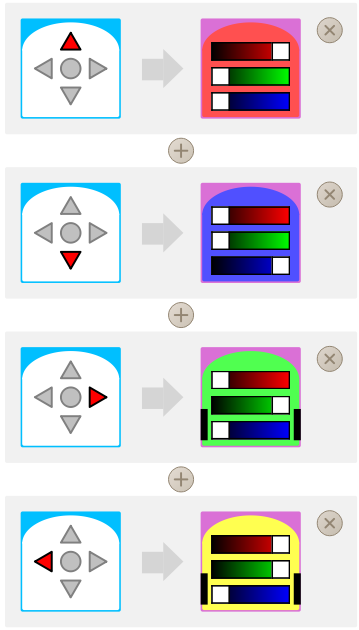
\includegraphics[width = 0.4\textwidth]{colors1}
	}
    \hspace{1.5cm}
    \subfigure[Éteindre Thymio lorsque le bouton centrale est touché]{
		\label{fig.colors-b}
		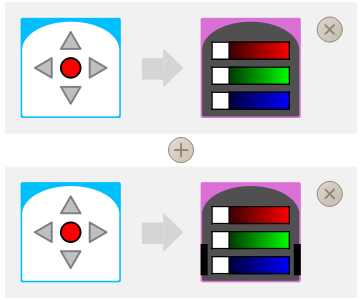
\includegraphics[width = 0.4\textwidth]{colors2-1-3}
	}
    \caption{Jouer avec les lumières de Thymio}
    \label{fig.colors}
\end{figure}
